\documentclass[12pt]{report}
\pagenumbering{roman}

\usepackage{graphicx}
\usepackage{subcaption}
\usepackage[utf8]{inputenc}
\usepackage[german]{babel}
% for units
\usepackage{siunitx}
% floats pictures to the correct position when using [H]
\usepackage{float}

\usepackage{hyperref}
\hypersetup{
  colorlinks=true,
  linkcolor=blue,
  filecolor=magenta,      
  urlcolor=cyan,
}

\urlstyle{same}


\begin{document}
% CONSTANTS BEGIN
\newcommand{\paragraphwithnewline}[1]{\paragraph{#1}\mbox{}\\} % used to create a newline after the paragraph tag.
\newcommand{\githubrepo}{\href{https://github.com/Pierrefha/ees-buggy-project}{GitHub-Repository}}
\newcommand{\referenzcode}{\href{https://github.com/tomfclarke/adafruit-motor-hat-cpp-library}{Referenz-Code}}
% \newcommand{\github_repo}{\href{https://github.com/Pierrefha/ees-buggy-project}{GitHub-Repository}}
% \newcommand{\referenz_code}{\href{https://github.com/tomfclarke/adafruit-motor-hat-cpp-library}{Referenz-Code}}
% CONSTANTS END
\begin{titlepage}
    \begin{center}
        \vspace*{1cm}
            
        \Huge
        \textbf{Lernportfolio}

        \vspace{1.5cm}
            
        \normalsize
        \textbf{Pierre Dahmani pd1528s 3215892\\
        Jens Peter Dennigmann jd8389s 3190025 \\
        Leonhard Kipp lk2149s 3188047\\}
            
        \vfill
            
        EES Buggy-Projekt 
        \vspace{0.8cm}
            
        %% TODO Add title pic
        %% \includegraphics[width=0.4\textwidth]{university}
        \pagebreak
    \end{center}
\end{titlepage}

% TODO Inhaltsverzeichnis

\begin{section}{Aufbau des Buggy}

\begin{figure}[h!]
  \centering
  \captionsetup[subfigure]{labelformat=empty}
  \begin{subfigure}{0.45\linewidth}
    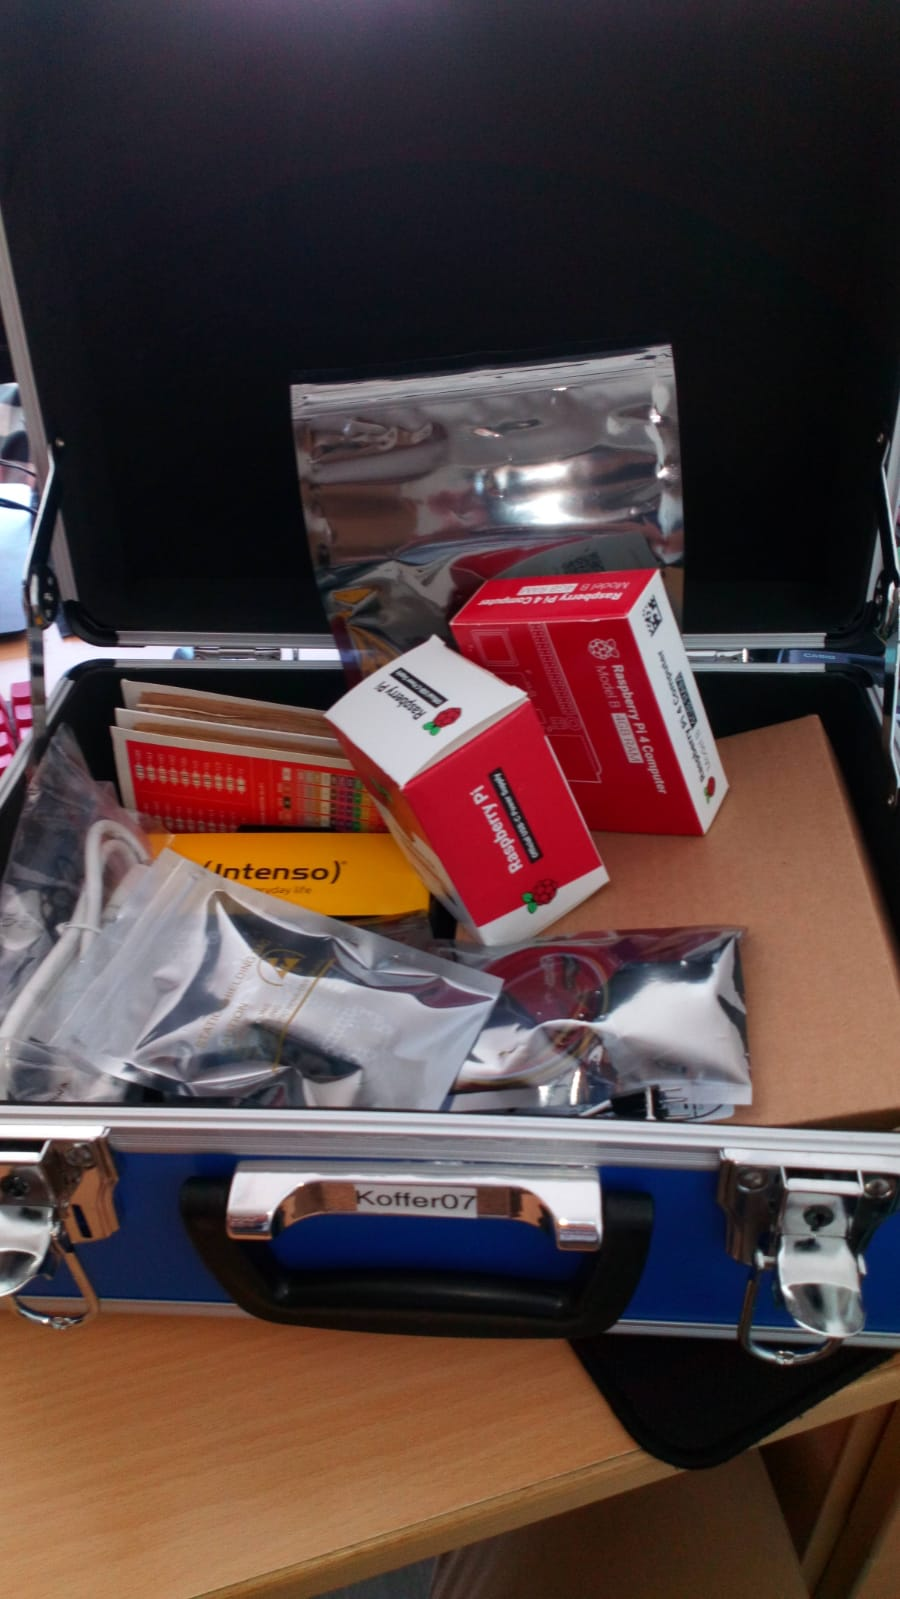
\includegraphics[width=\linewidth]{lernportfolio_assets/Buggy_Koffer.jpeg}
    \caption{Der Buggy vor dem Aufbau.}
  \end{subfigure}
  \begin{subfigure}{0.45\linewidth}
    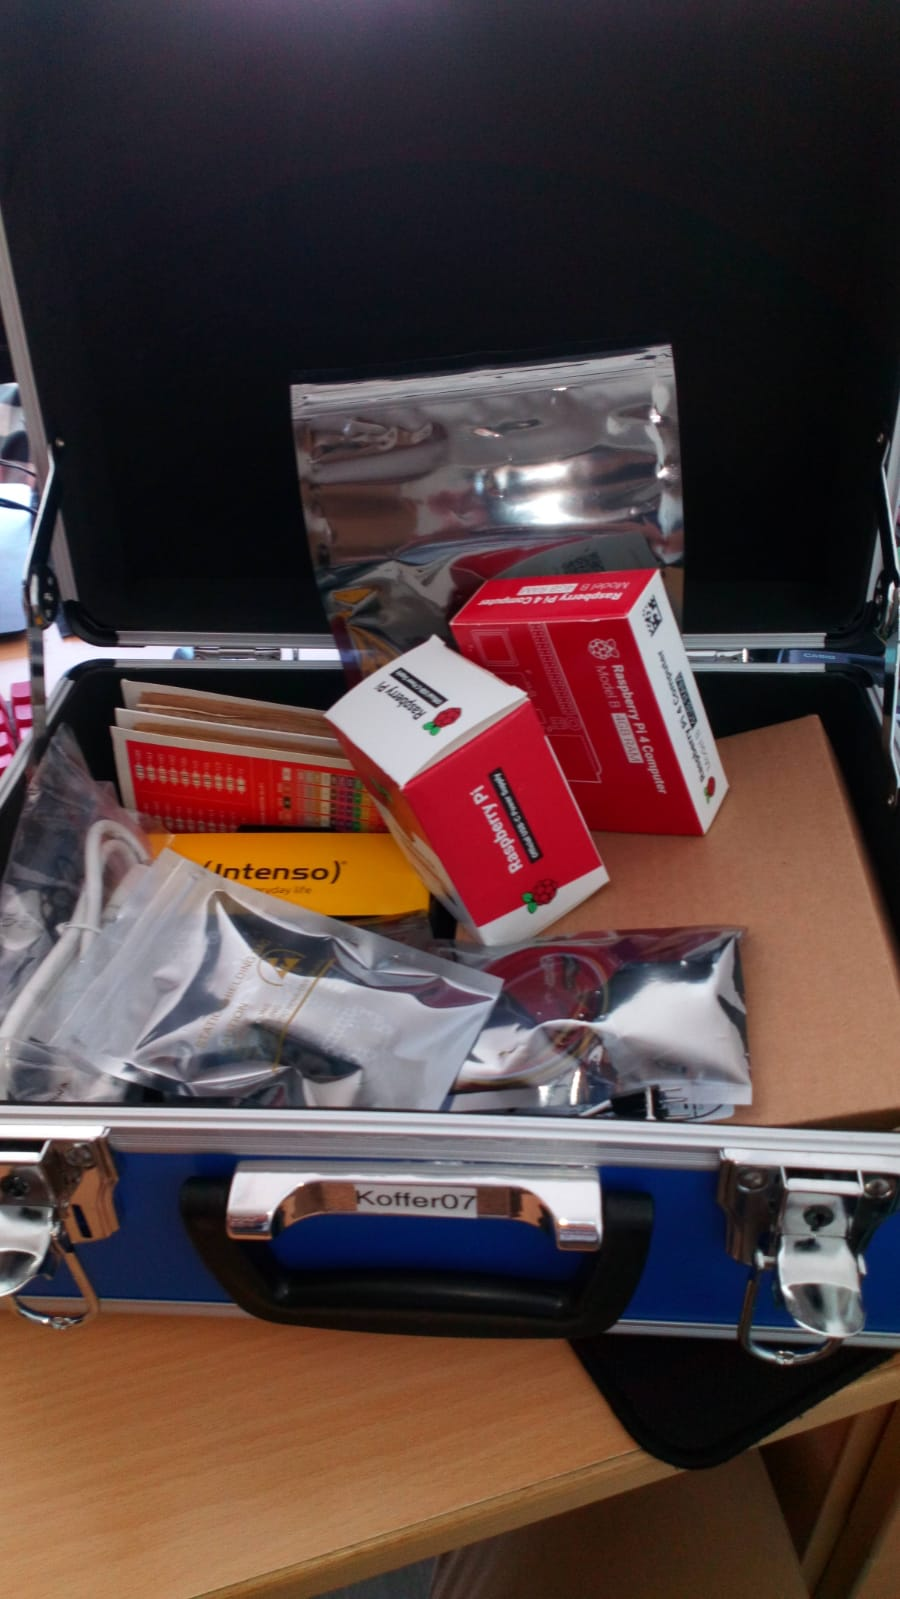
\includegraphics[width=\linewidth]{lernportfolio_assets/Buggy_Koffer.jpeg}
    \caption{Und danach.}
  \end{subfigure}
\end{figure}

Der Buggy wurde vor der Herausgabe des Arbeitsauftrages zusammengebaut. Zwischenschritte sind daher nicht bildlich festgehalten. 

Der Zusammenbau des Buggies verlief problemlos. Der Text ist insgesamt verständlich geschrieben und war eine große Unterstützung.

% Wollen wir das aufnehmen?
% Im Text ist der Genetiv von ``der Buggy'' durchgehend ``des Buggies''. Mit Verweis
% auf \url{https://www.duden.de/rechtschreibung/Buggy} ist der korrekte - und
% kontraintuitive - Genetiv ``des Buggys''.
In den meisten Bildern (außer auf Seite IV) ist der Buggy mit roter Platte gezeigt, wenngleich die Anleitung hier den weißen Winkel vorsieht. Eine Anmerkung, dass der Buggy im Folgendem mit roter Platte statt Winkel gezeigt wird, hätte eine kurze Verwirrung meinerseits verhindert.

Als Ubuntu-Nutzer bzw. Linux-Nutzer muss man keine zusätzliche Software installieren um eine SSH-Verbindung herzustellen. Eine Ergänzung, dass \href{https://invisible-island.net/xterm/}{XTerm} eine Empfehlung an die Windows-Nutzer ist, wäre daher angebracht. Bei dieser Bemerkung wird davon ausgegangen, dass mit XTerm an dieser Stelle \href{https://mobaxterm.mobatek.net/}{MobaXterm} gemeint ist und nicht der Terminal Emulator XTerm. 

Für den kompletten Zusammenbau wurden insgesamt 1,5 Stunden benötigt.

%Das meinst du nicht ernst oder ??? Ich bin dafür das kommt raus.
% Das ist der Punkt 1.4 aus  Arbeitsauftrag Projektphase_EES.pdf? 
Weil der Buggy schon vor Herausgabe des Arbeitsauftrages und während der anhaltenden Corona Phase abgeholt worden ist, wurde der Buggy von einer Person aufgebaut. Im Nachhinein haben wir uns trotzdem Gedanken dazu gemacht, wie wir den Aufbau am besten hätten aufteilen können. Wir sind zu dem Ergebnis gekommen, dass jede Person einen Teil des Buggys aufbauen sollte. Konkret hätte sich einer um das Kugellager und die Motoren gekümmert. Einer um die Abstandhalter und das Anbringen der Plastikplatte und des Raspberry Pi. Der letzte um das Anbringen des Motorhats und um das Anschließen und Fixieren der Powerbank.

\end{section}

\begin{section}{Motorensteuerung}

  Videos zu den Tests der Motorensteuerung sind unter: TODO LINK EINFÜGEN
  Der Quelltext kann unter \githubrepo{} eingesehen werden.

  Die Aufgabenstellung wurde so verstanden, dass man die Motorensteuerung
  selbst implementieren sollte. Das Lösen der Aufgabe geschah vor Erscheinen des
  erklärenden Forenposts. Daher wird im Folgendem auch über das Erstellen des
  Motorentreibers reflektiert.

  Herausforderungen bei der Programmierung waren vor allem 4 Punkte: 1. Finden der wichtigen
  Dokumentation, 2. Verstehen der Dokumentation, 3. Extraktion der relevanten
  Informationen und 4. Analyse des Beispielcodes.

  Der Motorhat ist mit dem RaspberryPi über I<sup>2</sup>C verbunden. Die
  Wiring Pi Bibliothek ermöglicht das Verbinden, Schreiben und Lesen von
  Registern über dieses Protokoll auf komfortablem und leicht verständlichem Wege.
  Bei der Benutzung dieser Bibliothek kam es zu keinen Problemen.
  
  Durch die Schematas unter
  \url{https://learn.adafruit.com/adafruit-dc-and-stepper-motor-hat-for-raspberry-pi/downloads}
  konnte die Verknüpfung der Pins des PCA9685 PWM LED Controllers mit den beiden
  TB6612FNG Motorsteuerungschips nachvollzogen werden.
  Durch die Datenblätter wurde die Funktionsweise des '\referenzcode's
  verständlich, wenngleich hierbei eine Frage offengeblieben ist:
  Der Referenzcode schreibt den Wert 4096 in ein LED On bzw. Off Register um den
  jeweiligen Motor an bzw. auszuschalten. In der Dokumentation des PCA9685 PWM LED
  Controllers heißt es jedoch unter Punkt 7.3.4 : ``The LEDn\_ON and LEDn\_OFF
  counts can vary from 0 to 4095.''.

  In den ersten Testläufen hat sich der Buggy beim Forwärtsfahren im Kreis
  gedreht. Die Motoren haben in unterschiedliche Richtungen gedreht. Dieses
  Verhalten war verständlich, da beide Motoren auf forwärts gestellt waren, was
  synonym für eine rechtsläufige Bewegung war. Für das rechte Rad bedeutet
  'rechtsläufig' forwärts. Für das linke Rad, welches durch den Anbau 
  \ang{180} um die Z-Achse gedreht ist, bedeutet dies rückwärts.
  Das Problem konnte behoben werden, indem die beiden Pins, welche für die Richtung
  zuständig sind, vertauscht wurden. So wurde jede rechtsläufige Bewegung zu einer
  linksläufigen und vice versa. Ein Forwärts-Kommando an das linke Rad wurde nun
  korrekterweise automatisch in eine linksläufige Bewegung übersetzt.
  Weiterhin war es ein Problem den Buggy konsistent losfahren zu lassen. Niedrige 
  Geschwindigkeit sind beim Start zu gering, um die Motoren drehen zu
  lassen. Das hat dazu geführt, dass der Buggy oft nicht losfuhr, trotz eines
  forwärts Kommandos. Dieses Problem konnte behoben werden, indem eine Mindestgeschwindigkeit
  eingestellt worden ist, sodass der Buggy nicht mit niedrigen Geschwindigkeiten
  konfigurierbar ist.

  Neben den technischen Herausforderungen war auch das Testen des Codes auf dem
  Raspberry Pi eine Umgewöhnung. Der Code konnte nicht lokal (auf dem eigenen
  Rechner) getestet werden, da die WiringPi Bibliothek nur auf einem Raspberry Pi funktioniert.
  Als Workflow hat sich durchgesetzt, dass auf dem eigenen Rechner entwickelt
  wurde, die Änderungen commitet und in das \githubrepo gepusht worden sind.
  Danach wurde der neue Code auf dem Raspberry Pi runtergeladen, die Binary
  durch ``cmake . \&\& make'' gebaut und schließlich getestet. Kleine Änderungen
  wurden auf dem Raspberry Pi durch den Texteditor Vim vollzogen.

  Besonders hilfreich war zur Lösung dieser Aufgabe, die Vertrautheit im Umgang
  mit Datenblättern, die man aus der Vorlesung bzw. Praktikum mitgenommen hat.
  Das Verstehen der Registertabellen fiel deutlich einfacher als beim ersten
  mal und das Unterscheiden zwischen wichtigen und unwichtigen Informationen
  ging schneller.

    TODO Video einfügen von der Rechteckfahrt objects/rectangle.mp4

\end{section}

\begin{section}{Ultraschallsteuerung}
    % START task 3.1 of Arbeitsauftrag Projektphase_EES.pdf
    \begin{subsection}{Recherche zum Ultraschallsensor und der Entfernungsmessung}
        Bei der Suche nach einem Datasheet zum HC-SR04 haben wir vergeblich nach
        einem offiziellen Datasheet gesucht. Daher haben wir uns  verschiedene 
        Datasheets zum HC-SR04 angeschaut und die Spezifikationen gründlich
        miteinander verglichen um sicher zu gehen, dass die Werte stimmen.
        Um auf eine Formel für die Distanzberechnung mithilfe von Ultraschall
        zu kommen haben wir nach der Geschwindigkeit von Schall in Luft gesucht.
        Dadurch können wir nun mit Hilfe des Sensors die Distanz des Buggys zum
        nächsten Objekt mit folgender Formel berechnen:\\
        Distanz in \si\cm = \( \frac{Signalzeit}{2} \) \si{\milli\second} $ \times $ 34.3 \si[per-mode = fraction]{\cm\per\milli\second}
        

        % paragraph can be used for captions inside subsections
        \begin{paragraph}{Quellen}
        \begin{itemize}
            \item \url{https://www.electroschematics.com/hc-sr04-datasheet}
            \item \url{https://components101.com/ultrasonic-sensor-working-pinout-datasheet}
            \item \url{https://www.sparkfun.com/products/15569\#documents-tab}
            \item \url{https://en.wikipedia.org/wiki/Speed\_of\_sound}
            \item \url{http://www.sengpielaudio.com/calculator-speedsound.htm}
        \end{itemize}
        \end{paragraph}
    \end{subsection}
    % END task 3.1

    % START task 3.3 of Arbeitsauftrag Projektphase_EES.pdf
    \begin{subsection}{Steuerung und Auslesen von GPIOs}
        % Was haben Sie über die Steuerung und Auslesen von GPIOs gelernt
        % und welches Wissen und Techniken aus dem ersten Teil der Vorlesung
        % konnten Sie einsetzen?
        Dank der Vorlesung haben wir gelernt, dass die GPIO Pins verschiedene
        Modi besitzen. Um Signale zu senden muss man sie in den Output-Mode 
        versetzen. Wenn man Signale empfangen will muss man den Pin in
        den Input-Mode versetzten. Hier haben wir gelernt wie wichtig es ist 
        auch die korrekte Spannung angelegt zu haben! Sowohl beim STM32 als auch
        beim Raspberry Pi darf die Eingangsspannung 3.3V nicht überschreiten.
        Höhere Eingangsspannungen (wie etwa die 5V die vom Ultraschallsensor 
        ausgehen) können das Gerät zerstören! Wir haben ebenfalls gelernt, 
        dass es zu einem floating State kommen kann, wenn wir keine Pull-up 
        bzw. Pull-down Widerstände einsetzen. Dies kann bei der 
        Nachimplementierung für bestimmte Protokolle genutzt werden. Bei unserem
        Anwendungsfall gilt es jedoch, diese zu verhindern und klare Low und High
        Pegel zu erhalten.\\
        Mit unseren Kenntnissen konnten wir nun einen Schaltplan anfertigen:
        % testing figure
        \begin{figure}[H]
        \centering
            \begin{minipage}{0.45\textwidth}
                \centering
                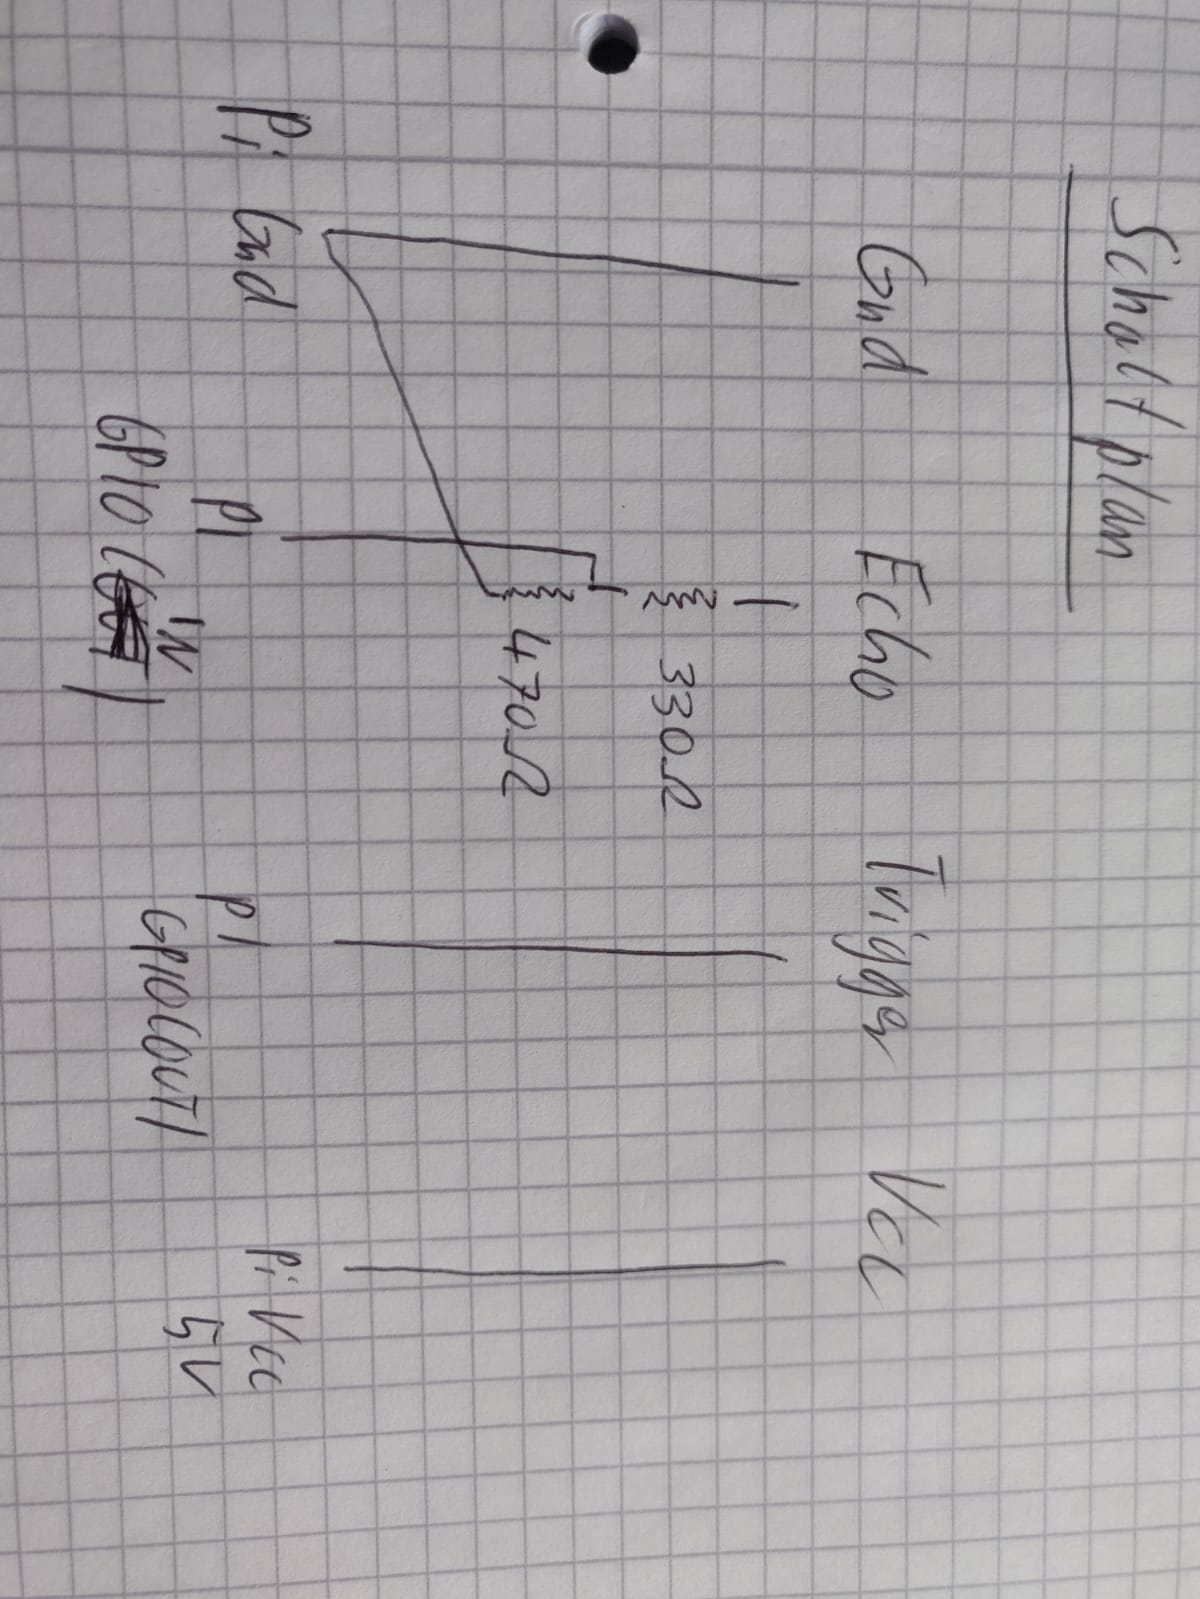
\includegraphics[width=0.9\textwidth]{lernportfolio_assets/Schaltplan_Ultraschallsensor1}
                \caption{Auf Papier geplant}
            \end{minipage}
            \centering
            \begin{minipage}{0.45\textwidth}
                \centering
                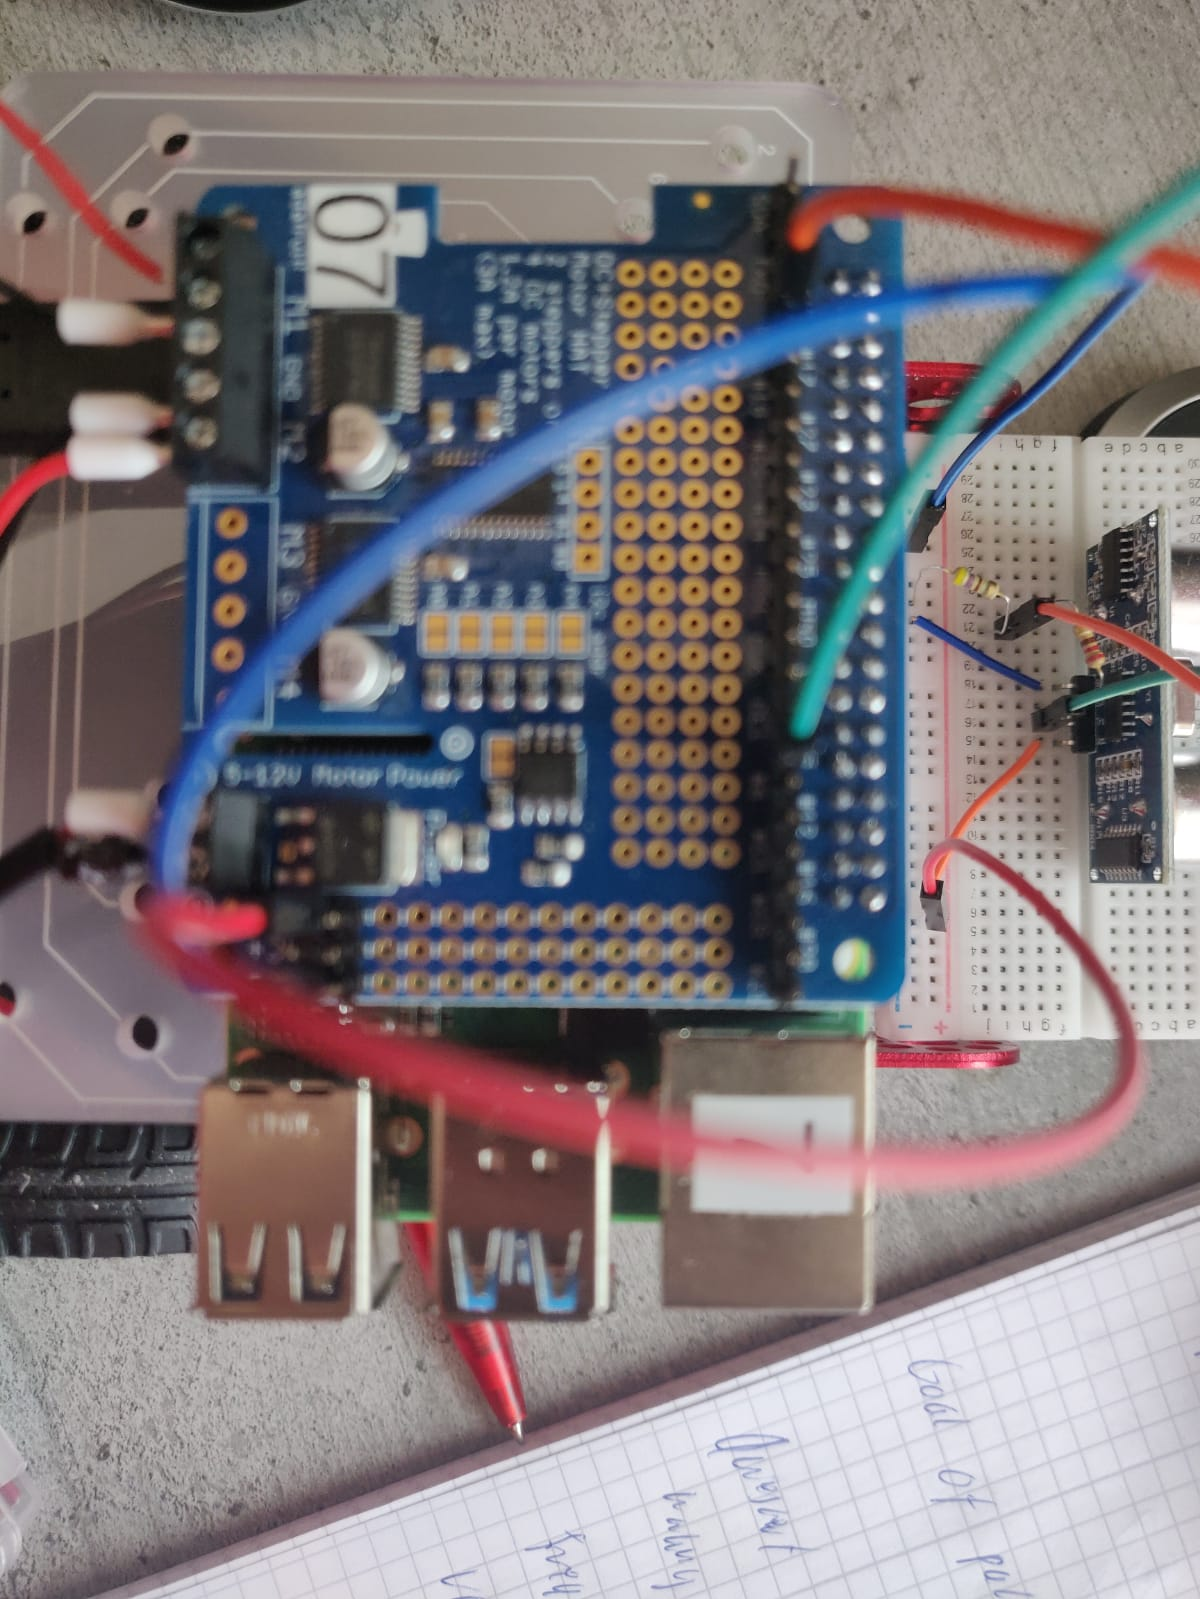
\includegraphics[width=0.9\textwidth]{lernportfolio_assets/Schaltplan_Ultraschallsensor2} 
                \caption{Im Buggy verbaut}
            \end{minipage}
        \end{figure}

    \end{subsection}
    % END task 3.3

    % START task 3.4 of Arbeitsauftrag Projektphase_EES.pdf
    \begin{subsection}{Stolpersteine bei der Programmierung}
        % Erörtern Sie, was bei der Programmierung der Entfernungsmessung
        % mit dem Ultraschallsensor besonders wichtig ist.
        Durch das Einbinden des Ultraschallsensors in unser Program sind wir auf
        einige Fehlerquellen gestoßen. Im folgenden erläutern wir die Lösunen zu
        unseren Problemen.
        \begin{paragraphwithnewline}{Theorie und Praxis}
            Laut Datenblatt muss der Trigger pin für mindestens 10 \si{\micro\second}
            auf High gesetzt werden um die Ultraschallwelle auszulösen. Dadurch
            hat man bei manchen Messungen jedoch kein Signal beim Trigger erzeugt
            und hat dadurch komplett falsche Werte erhalten. Hier hat sich
            schnell gezeigt, dass es in der Praxis besser ist eine gewisse Fehlertoleranz
            einzubauen. Den Wert auf 20\si{\micro\second} zu erhöhen hat unser
            Problem dann gelöst.
        \end{paragraphwithnewline}

        \begin{paragraphwithnewline}{Falsche Messwerte filtern}
            Durch Störungen wird der Ultraschallsensor auch ggfs. falsche Werte
            erzeugen. Um das Messergebnis nicht zu verfälschen muss man einen
            Mechanismus einfügen der überprüft, ob die erhaltenen Werte wirklich
            sinnvoll sind. 
        \end{paragraphwithnewline}

        \begin{paragraphwithnewline}{Distanz möglichst genau berechnen}
            Die Messvarianz kann bei einzelnen Messungen das Ergebnis stark
            beeinflussen. Um dem entgegenzuwirken wird die Messung mehrmals
            wiederholt und die Distanz auf Basis des Mittelwerts gebildet.
        \end{paragraphwithnewline}

        % backup text that will be deleted when finished.
        % Durch das Einbinden des Ultraschallsensors in unser Program sind wir auf
        % einige Fehlerquellen gestoßen. Um den Trigger und damit die Ultraschall
        % welle auszulösen muss der Pin für mindestens 10 \si{\micro\second} auf
        % High gesetzt werden. Dies hatten wir zu Beginn eingestellt. Doch wir haben
        % schnell gemerkt, dass manche Messungen nicht zustande gekommen sind, weil
        % beim Echo Pin keine Antwort angekommen ist. Dadurch haben wir gelernt, 
        % dass es in der Praxis doch besser ist auf Nummer sicher zu gehen und 
        % haben dieses Zeitfenster auf 20 \si{\micro\second} erhöht. Unser nächstes
        % Problem bestand darin, dass einzelne Messungen starke Abweichungen zum 
        % Referenzwert aufwiesen. Dieses Problem wollten wir dadurch lösen, dass wir
        % anstatt einer Messung nun 30 Messungen vornehmen und den Durchschnitt der
        % erhaltenen Werte zurückgeben. Doch nun kam es zu sehr starken, unlogischen
        % Abweichungen. Dies kam zu stande weil wir nach einer Messung nicht lange
        % genug gewartet hatten, bis sich zu Pins zu ihren korrekten Pegeln zurück
        % gesetzt hatten. Dieses Problem haben wir dadurch behoben, dass wir nun
        % nach jeder Messung 1 \si{\milli\second} warten. Durch Störfaktoren (z.B.
        % starker Wind) kann es ebenfalls zu komplett falschen Messwerten kommen,
        % die wir nicht in die Messung aufnehmen dürfen. Da der Ultraschallsensor
        % Distanzen im Berech von 4\si\cm bis 400\si\cm Messen kann nehmen wir 
        % Messergebnisse, die eine errechnete Distanz von 3.5\si\cm unterschreiten,
        % nicht mit in die Messung auf.

    \end{subsection}
    % END task 3.4

    % START task 3.5 of Arbeitsauftrag Projektphase_EES.pdf
    \begin{subsection}{Bewertung der Zuverlässigkeit der Entfernungsmessung}
      Die Entfernungsmessung funktioniert für solide Objekte in einer Reichweite
      von 5 bis 100 cm zuverlässig. Für weniger solide Objekten, wie z.B. einer
      Pappierbox, hat der Sensor bei den Tests Probleme
      gehabt, die Entfernung richtig einzuschätzen. Oftmals kam es hierbei zu keinen Rückmeldungen an den Echo-Pin. Dieses
      Problem wurde durch ein Zeitlimit beim Warten auf den Echo-Pin gelöst und
      verwerfen der Messung falls das Zeitlimit überschritten wurde. Das
      Ermitteln der Entfernung beinhaltet mehrere Entfernungsmessungen. Somit
      ist das verwerfen einzelner Messungen durch ein überschreiten des
      Zeitlimits vertretbar. Aus den Messungen wird anschließend ein Mittelwert
      gebildet und zurückgegeben. Durch mehrmaliges Messen und bilden des
      Mittelwertes wird zugleich die relativ hohe Varianz zwischen einzelnen
      Messungen bei gleicher Distanz zum Objekt abgefangen.
    \end{subsection}
    \begin{subsection}{Bewertung der Genauigkeit}
      Die Entfernungsmessung funktioniert mit einer Standardabweichung von unter
      1,3 cm auf 100 cm genau.
      Die Rohdaten können im Anhang \ref{ultraschallsensorRohdaten} eingesehen werden.
      Im folgendem eine Zusammenfassung.
      %The table is generated by pandas
      \begin{table}[h!]
        \begin{tabular}{lrrrrrrr}
          % \toprule
          Abstand &       5cm &        10cm &        15cm &        20cm &        30cm &        50cm &       100cm \\
          % \midrule
          count &  100.000000 &  100.000000 &  100.000000 &  100.000000 &  100.000000 &  100.000000 &  100.000000 \\
          mean  &    4.668009 &    9.355380 &   13.951283 &   19.938128 &   30.418109 &   51.078758 &   99.553521 \\
          std   &    0.032030 &    0.305832 &    0.109583 &    0.060932 &    0.107799 &    0.482031 &    1.268841 \\
          min   &    4.650300 &    8.792790 &   13.804400 &   19.811500 &   30.079000 &   50.054500 &   91.353200 \\
          25\%   &    4.663265 &    9.122402 &   13.854150 &   19.880775 &   30.405600 &   50.820775 &   99.667750 \\
          50\%   &    4.664025 &    9.305280 &   13.912850 &   19.933800 &   30.450700 &   50.999200 &   99.878350 \\
          75\%   &    4.665242 &    9.658680 &   14.020900 &   19.983375 &   30.478350 &   51.518525 &   99.959425 \\
          max   &    4.979740 &    9.821430 &   14.231100 &   20.131400 &   30.566800 &   51.951700 &  100.912000 \\
          % \bottomrule
        \end{tabular}
        \caption{Zusammenfassung der Rohdaten. Alle Werte in cm.}
    \end{table}
    Aus der Tabelle geht hervor, dass der Abstand zu nahen
    Objekten (Abstand <= 20 cm) tendenziell unterschätzt wird, zu entfernteren
    Objekten hingegen geringfügig überschätzt. Eine Ausnahme bildet hier die
    Messreihe für den Abstand von 100 cm.
    
    Um den Mittelwert gibt es für alle Werte eine Standardabweichung von weniger
    als 1,3 cm. Die Messung sind daher präzise. Erwähnenswert ist, dass die
    Standardabweichung bei kleineren Distanzen sehr viel geringer ist als bei größeren.

    \begin{figure}[h!]
      \centering
      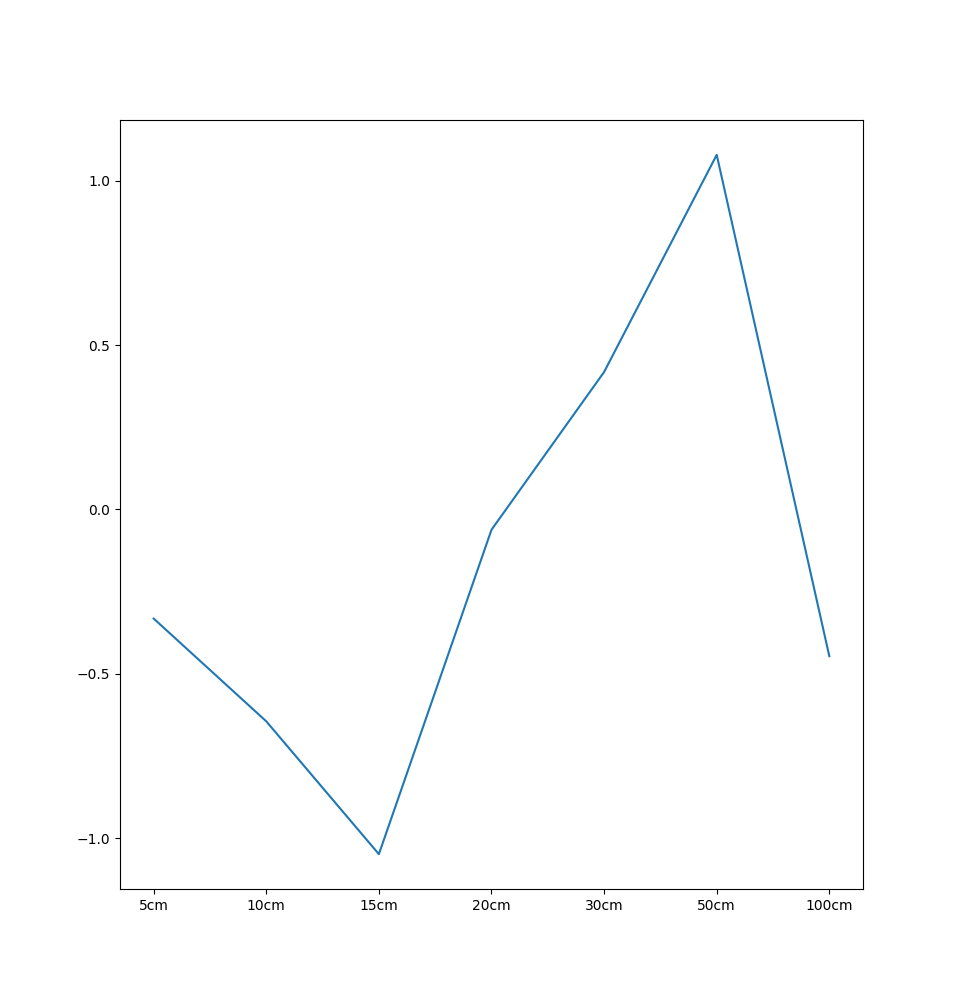
\includegraphics[width=0.5\textwidth]{test_data_ultrasonic/meanDiff.png}
      \caption{Differenz des Mittelwertes zur tatsächlichen Distanz}
    \end{figure}

  \end{subsection}
  % END task 3.5


\end{section}

\begin{section}{Kompass}
  \begin{subsection}{Analyse der Genauigkeit}
  \end{subsection}
\end{section}


\begin{section}{Anhang}
  \begin{subsection}{Rohdaten Ultraschallsensor} \label{ultraschallsensorRohdaten}
    \input{test_data_ultrasonic/rohdaten.tex}
  \end{subsection}
\end{section}

\end{document}

 
